
\documentclass[tikz,border=3pt]{standalone}
\usetikzlibrary{arrows.meta,positioning}
\begin{document}
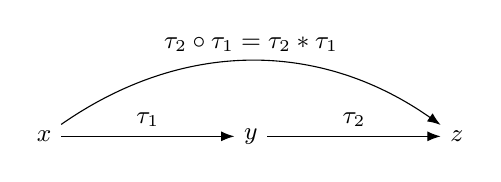
\begin{tikzpicture}[node distance=2.2cm, every node/.style={font=\small}]
\node (x) {$x$};
\node[right=of x] (y) {$y$};
\node[right=of y] (z) {$z$};
\draw[-{Latex}] (x) -- node[above] {$\tau_1$} (y);
\draw[-{Latex}] (y) -- node[above] {$\tau_2$} (z);
\draw[-{Latex}, bend left=35] (x) to node[above] {$\tau_2\circ\tau_1=\tau_2*\tau_1$} (z);
\end{tikzpicture}
\end{document}
